\documentclass[10pt,a4paper]{article}
\usepackage[a4paper,left=18mm,right=18mm,top=16mm,bottom=16mm]{geometry}
\usepackage{amsmath,amssymb}
\usepackage{booktabs}
\usepackage{graphicx}
\usepackage[expansion=false]{microtype}
\usepackage{siunitx}
\usepackage{caption}
\usepackage{capt-of}
\usepackage{xcolor}
\usepackage{fancyhdr}
\usepackage{titlesec}
\usepackage{enumitem}

\sisetup{detect-weight=true,detect-family=true,group-separator={,},
         group-digits=integer,group-minimum-digits=4}

\definecolor{accent}{HTML}{2F5D7C}
\definecolor{slate}{HTML}{4A5568}
\definecolor{green2}{HTML}{2F6D4F}
\definecolor{warm}{HTML}{B5553F}

\titleformat{\section}{\normalsize\bfseries\color{accent}}{}{0pt}{}
\titlespacing*{\section}{0pt}{12pt}{4pt}

\captionsetup{font=small,labelfont=bf,skip=3pt}
\captionsetup[table]{position=top}
\captionsetup{width=0.93\textwidth}

\pagestyle{fancy}\fancyhf{}
\fancyhead[L]{\small\color{slate} Results pack --- J.\ Mohindra, z5418455}
\fancyhead[R]{\small\color{slate}\thepage}
\renewcommand{\headrulewidth}{0.4pt}

\setlength{\tabcolsep}{5pt}
\renewcommand{\arraystretch}{1.05}

\newcommand{\tno}[1]{\textbf{#1}}

\begin{document}

\begin{center}
\begin{minipage}{0.98\textwidth}\centering
{\Large\bfseries Results Pack}\\[3pt]
{\small Compression of radar range--FFT data on Kintex UltraScale+ ---
all measured results, 17 September 2026}\\[2pt]
{\footnotesize Jordan Mohindra (z5418455) \quad$\cdot$\quad
Dataset: ColoRadar cascade, 50 frames \quad$\cdot$\quad
Device: \texttt{xcku5p-ffvb676-2-e} @ \SI{100}{\mega\hertz}}
\end{minipage}
\end{center}
\vspace{2pt}\hrule\vspace{6pt}

\noindent\footnotesize
\textbf{Reading guide.} Four designs appear throughout:
\textbf{DRHE-1} and \textbf{LPC-1,2} are the algorithms as originally
implemented (predicting from the immediately preceding ramp);
\textbf{DRHE-$n$} and \textbf{LPC-$n$,$2n$} are the TDM-corrected versions
(predicting from the preceding ramp of the same transmitter, $n = n_{\mathrm{Tx}} = 12$).
\normalsize

% ================================================================
\section{1\quad Phase 1 --- MATLAB reference benchmark}

\begin{center}
\begin{minipage}{0.98\textwidth}\centering
\captionof{table}{Single frame (\texttt{frame\_0}), 16 RX, 190 reference detections.}
\centering\small
\begin{tabular}{@{}lrrrrr@{}}
\toprule
Algorithm & CR & FN (\%) & FDR (\%) & NF (dBFS) & SNR (dB)\\
\midrule
FP16          & 1.00 & 0.00  & 0.00 & $-105.858$ & 36.256\\
DRHEfp16      & 1.05 & 0.00  & 0.00 & $-105.858$ & 36.256\\
FX16          & 1.00 & 3.68  & 0.00 & $-105.591$ & 36.150\\
\tno{DRHE}    & \tno{3.32} & 3.68 & 0.00 & $-105.591$ & 36.150\\
BAQ           & 3.76 & 4.74  & 3.72 & $-106.039$ & 36.562\\
RDVLE         & 1.12 & 20.53 & 2.58 & $-102.476$ & 33.791\\
RDVLE\_UDRE   & 2.56 & 26.32 & 2.78 & $-102.002$ & 33.663\\
\tno{LPC}     & \tno{3.39} & 3.68 & 0.00 & $-105.591$ & 36.150\\
\bottomrule
\end{tabular}
\end{minipage}
\end{center}

\begin{center}
\begin{minipage}{0.98\textwidth}\centering
\captionof{table}{50-frame average, 16 RX, \num{9934} reference detections. \emph{This is
the headline benchmark.} FX16, DRHE and LPC share detection metrics by
construction --- all three reconstruct the quantised data exactly.}
\centering\small
\begin{tabular}{@{}lrrrrr@{}}
\toprule
Algorithm & CR & FN (\%) & FDR (\%) & NF (dBFS) & SNR (dB)\\
\midrule
FP16          & 1.00 & 0.00  & 0.00 & $-105.638$ & 35.504\\
DRHEfp16      & 1.04 & 0.05  & 0.01 & $-105.637$ & 35.505\\
FX16          & 1.00 & 3.77  & 1.11 & $-105.374$ & 35.359\\
\tno{DRHE}    & \tno{3.30} & 3.77 & 1.11 & $-105.374$ & 35.359\\
BAQ           & 3.76 & 10.44 & 9.69 & $-105.080$ & 35.081\\
RDVLE         & 1.12 & 24.01 & 4.62 & $-102.275$ & 33.165\\
RDVLE\_UDRE   & 2.56 & 28.73 & 4.44 & $-101.782$ & 33.004\\
\tno{LPC}     & \tno{3.37} & 3.77 & 1.11 & $-105.374$ & 35.359\\
\bottomrule
\end{tabular}
\end{minipage}
\end{center}

% ================================================================
\section{2\quad Phase 2 --- bit-exact verification in hardware simulation}

\begin{center}
\begin{minipage}{0.98\textwidth}\centering
\captionof{table}{Vitis HLS C-simulation, all 50 frames, 4 RX, \num{157286400} complex
samples. \textbf{Every design reconstructs every sample exactly.}}
\centering\small
\begin{tabular}{@{}lrrrr@{}}
\toprule
Design & Mean CR & MaxDiff & MSE & Frames lossless\\
\midrule
DRHE-1          & \num{3.30987} & 0 & 0 & 50 / 50\\
\tno{DRHE-$n$}  & \tno{\num{3.75082}} & \tno{0} & 0 & 50 / 50\\
LPC-1,2         & \num{3.38497} & 0 & 0 & 50 / 50\\
\tno{LPC-$n$,$2n$} & \tno{\num{3.69681}} & \tno{0} & 0 & 50 / 50\\
\bottomrule
\end{tabular}
\end{minipage}
\end{center}

\begin{center}
\begin{minipage}{0.98\textwidth}\centering
\captionof{table}{Agreement between MATLAB and hardware. For LPC the entire residual
difference is AXI packet padding --- the underlying bit counts are identical.}
\centering\small
\begin{tabular}{@{}lr@{}}
\toprule
Quantity & Value\\
\midrule
LPC: MATLAB, double-precision coefficients      & \num{3.38541}\\
LPC: MATLAB, 16-bit quantised coefficients      & \num{3.38541}\\
\quad cost of coefficient quantisation          & \SI{0.0000}{\percent}\\
LPC: MATLAB, quantised + 256-bit AXI padding    & \tno{\num{3.38497}}\\
LPC: Vitis HLS measured                         & \tno{\num{3.38497}}\\
\quad frames where the padding model matches    & \num{50} / \num{50} (to $4.9\times10^{-6}$)\\
\quad worst single frame                        & \num{0.00091} \ (tolerance $\pm 0.01$)\\
\midrule
DRHE: hardware bits above MATLAB, per frame     & \num{15}--\num{252} (mean \num{134})\\
\quad one AXI packet                            & \num{256} bits\\
\bottomrule
\end{tabular}
\end{minipage}
\end{center}

% ================================================================
\section{3\quad Phase 2.4 --- synthetic edge cases}

\begin{center}
\begin{minipage}{0.98\textwidth}\centering
\captionof{table}{DRHE, 8 synthetic cases. The first run exposed the $-32768$ defect
(3 failures); after the saturation + closed-loop fix all 8 pass. The
\texttt{random-int16} case is the proof the closed loop works --- the clamp
fires repeatedly across all 192 ramps and the error still never exceeds 1 LSB.}
\centering\small
\begin{tabular}{@{}llrrrl@{}}
\toprule
Case & Input & CR & \multicolumn{2}{c}{MaxDiff} & Result\\
\cmidrule(lr){4-5}
 & & & before & after & \\
\midrule
all-zeros       & every sample 0                & 4.0000 & 0 & 0 & PASS\\
dc-constant     & Re=1000, Im=$-$500 everywhere & 3.5867 & 0 & 0 & PASS\\
random-int16    & uniform random int16          & 0.6037 & \textcolor{warm}{60475} & \tno{1} & PASS\\
tone-192ramp    & correlated tone, 192 ramps    & 3.2777 & 0 & 0 & PASS\\
tone-1ramp      & same tone, 1 ramp             & 0.6214 & 0 & 0 & PASS\\
max-amplitude   & all $+32767$                  & 3.0132 & 0 & 0 & PASS\\
max-alternating & $+32767 / -32768$ per ramp    & 3.0326 & \textcolor{warm}{65535} & \tno{1} & PASS\\
int16-min       & all $-32768$                  & 3.0371 & \textcolor{warm}{65535} & \tno{1} & PASS\\
\bottomrule
\end{tabular}
\end{minipage}
\end{center}

\begin{center}
\begin{minipage}{0.98\textwidth}\centering
\captionof{table}{LPC, same 8 cases, all pass. LPC's ratios are lower on the synthetic
cases because the \num{32768}-bit coefficient table is charged whatever the data
does --- on \texttt{all-zeros} the residual bits are identical and the
\num{4.00} vs \num{3.84} gap is exactly that overhead.}
\centering\small
\begin{tabular}{@{}lrrl@{}}
\toprule
Case & CR & MaxDiff & Result\\
\midrule
all-zeros       & 3.8400 & 0 & PASS\\
dc-constant     & 3.3758 & 0 & PASS\\
random-int16    & 0.6000 & 0 & PASS\\
tone-192ramp    & 1.1006 & 0 & PASS\\
tone-1ramp      & 0.2771 & 0 & PASS\\
max-amplitude   & 0.9868 & 0 & PASS\\
max-alternating & 0.9868 & 1 & PASS\\
int16-min       & 0.9868 & 1 & PASS\\
\bottomrule
\end{tabular}
\end{minipage}
\end{center}

\noindent\footnotesize
\textbf{Note on \texttt{random-int16}.} CR $<1$ is correct behaviour, not a
fault: a Huffman/append coder cannot leave incompressible data unchanged, it
expands it. A deployment needs a raw-passthrough fallback if such data is
possible.\normalsize

% ================================================================
\section{4\quad Phase 3 --- synthesis and RTL co-simulation}

\begin{center}
\begin{minipage}{0.98\textwidth}\centering
\captionof{table}{Post-synthesis resources and timing, all four designs. Device
capacity: \num{216960} LUT, \num{433920} FF, \num{960} BRAM\_18K, \num{1824}
DSP. Frame latency is measured in RTL co-simulation, not estimated.}
\centering\small
\begin{tabular}{@{}lrrrrr@{}}
\toprule
& DRHE-1 & DRHE-$n$ & LPC-1,2 & LPC-$n$,$2n$ & Kiem (ZU3EG)\\
\midrule
LUT              & \num{115532} & \num{115736} & \num{80528} & \num{86298} & \num{45892}\\
\quad \% device  & 53\% & 53\% & 37\% & 40\% & 65\% (of ZU3EG)\\
FF               & \num{57105}  & \num{57263}  & \num{17393} & \num{23154} & \num{9243}\\
BRAM\_18K        & \num{40}     & \tno{\num{80}} & \num{256} & \tno{\num{192}} & \num{10}\\
DSP              & \num{132}    & \num{132}    & \num{168}   & \num{156} & \num{44}\\
Est.\ $F_{\max}$ & \SI{81.88}{\mega\hertz} & \SI{81.88}{\mega\hertz}
                 & \SI{85.43}{\mega\hertz} & \SI{85.43}{\mega\hertz} & \SI{100}{\mega\hertz}\\
Worst loop II    & 2 & 2 & 3 & \tno{1} & 1\\
Pipeline depth   & 58 & 58 & --- & --- & ---\\
Frame latency (cyc) & \num{61253} & \tno{\num{61253}} & \num{197277} & \num{325166} & ---\\
Frame buffer     & none & none & \SI{3.1}{\mebi bit} & \SI{3.1}{\mebi bit} & ---\\
\bottomrule
\end{tabular}
\end{minipage}
\end{center}

\begin{center}
\begin{minipage}{0.98\textwidth}\centering
\captionof{table}{Throughput. \textbf{Unit correction:} Kiem's published
\SI{11.92}{Gbit\per\second} is in \emph{gibibits}; $11.92 \times 2^{30} / 10^8 =
127.99$ bits/cycle, i.e.\ exactly \num{128} --- the full AXI bus width at
II\,=\,1. Its decimal equivalent is \SI{12.80}{Gbit\per\second}.}
\centering\small
\begin{tabular}{@{}lrrr@{}}
\toprule
& DRHE & LPC & Kiem (corrected)\\
\midrule
Effective II                        & 2 & 3 & 1\\
bits per cycle                      & 51.4 & 15.9 & \tno{128.0}\\
Throughput @ \SI{100}{\mega\hertz}  & \SI{5.14}{Gbit\per\second} & \SI{1.60}{Gbit\per\second} & \SI{12.80}{Gbit\per\second}\\
Throughput @ own $F_{\max}$         & \SI{4.21}{Gbit\per\second} & \SI{1.36}{Gbit\per\second} & ---\\
IP pipeline latency                 & \SI{580}{\nano\second} & --- & \SI{230}{\nano\second}\\
\bottomrule
\end{tabular}
\end{minipage}
\end{center}

\begin{center}
\begin{minipage}{0.98\textwidth}\centering
\captionof{table}{LPC-1,2 cycle breakdown. The model is accurate to
\SI{0.08}{\percent}. For LPC-$n$,$2n$ the same model predicts \num{246272}
against \num{325166} measured --- the \SI{32}{\percent} gap is pipeline drain
from \num{512} short loop invocations ($512 \times (71+56) \approx \num{65000}$
cycles).}
\centering\small
\begin{tabular}{@{}lrrr@{}}
\toprule
Stage & Iterations & II & Cycles\\
\midrule
Ingest            & \num{24576} & 3 & \num{73728}\\
Solve + residual  & \num{98304} & 1 & \num{98304}\\
Emit coefficients & \num{512}   & 1 & \num{512}\\
Emit residuals    & \num{24576} & 1 & \num{24576}\\
\midrule
Model total       & & & \num{197120}\\
\tno{Measured (co-simulation)} & & & \tno{\num{197277}}\\
\bottomrule
\end{tabular}
\end{minipage}
\end{center}

% ================================================================
\section{5\quad The audit --- what the compression ratio measures}

\begin{center}
\begin{minipage}{0.98\textwidth}\centering
\captionof{table}{\textbf{The no-prediction baseline.} Raw FX16 values coded through the
\emph{identical} S4 + Huffman back end with no predictor. 5 frames, 4 RX. Both
predictors as implemented perform \emph{worse} than doing nothing.}
\centering\small
\begin{tabular}{@{}lrrr@{}}
\toprule
Configuration & bits/value & CR & vs.\ no prediction\\
\midrule
\tno{No prediction (entropy coder only)} & \tno{4.586} & \tno{3.489} & ---\\
DRHE-1 (as implemented)                  & 4.821 & 3.319 & \textcolor{warm}{$0.951\times$}\\
LPC-1,2 (as implemented)                 & 4.710 & 3.397 & \textcolor{warm}{$0.974\times$}\\
\bottomrule
\end{tabular}
\end{minipage}
\end{center}

\begin{center}
\begin{minipage}{0.98\textwidth}\centering
\captionof{table}{Entropy check, independent of the coder. The predictor was
\emph{increasing} the information content of the data.}
\centering\small
\begin{tabular}{@{}lr@{}}
\toprule
Quantity & Value\\
\midrule
Order-0 entropy, raw FX16 codes        & \SI{4.094}{bits}\\
Order-0 entropy, DRHE-1 residuals      & \textcolor{warm}{\SI{4.538}{bits}}\\
Achieved bits/value, no prediction     & \SI{4.586}{bits}\\
Huffman overhead above entropy         & \SI{0.283}{bits} (\SI{6.2}{\percent})\\
\bottomrule
\end{tabular}
\end{minipage}
\end{center}

\begin{center}
\begin{minipage}{0.98\textwidth}\centering
\captionof{table}{\textbf{Decomposition of the compression ratio.} Most of it is unused
fixed-point container, not algorithm.}
\centering\small
\begin{tabular}{@{}lrl@{}}
\toprule
Source & Factor & Evidence\\
\midrule
Unused container headroom & $\times\,1.63$ & peak raw ADC sample \num{914} of \num{32767};\\
                          &                & peak FX16 code \num{436} $\Rightarrow$ \num{9.8} of \num{16} bits used\\
Spectral sparsity         & $\times\,2.14$ & $9.8 \rightarrow 4.59$ bits, genuine\\
\midrule
\tno{Subtotal, no prediction} & \tno{$\times\,3.489$} & \\
Prediction, as implemented    & \textcolor{warm}{$\times\,0.95$} & negative contribution\\
\tno{Prediction, corrected}   & \tno{$\times\,1.08$} & \\
\bottomrule
\end{tabular}
\end{minipage}
\end{center}

\begin{center}
\begin{minipage}{0.98\textwidth}\centering
\captionof{table}{\textbf{Prediction axis study.} 5 frames, 4 RX, 128 bins, 192 ramps.
Gain is relative to no prediction; below \num{1.000} means the predictor is
doing harm. Row 5 is the obvious alternative that fails: per-transmitter blocks
multiply the coefficient overhead by 12 (\SI{1.04}{\percent} $\rightarrow$
\SI{12.5}{\percent} of the frame) and shorten each fit from 192 samples to 16.}
\centering\small
\begin{tabular}{@{}lrrr@{}}
\toprule
Configuration & bits/value & CR & gain\\
\midrule
No prediction                                  & 4.586 & 3.489 & 1.000\\
DRHE, lag 1 \emph{(as implemented)}            & 4.821 & 3.319 & \textcolor{warm}{0.951}\\
\tno{DRHE, lag $n_{\mathrm{Tx}}$}              & \tno{4.240} & \tno{3.774} & \tno{1.082}\\
LPC, lags 1, 2 \emph{(as implemented)}         & 4.710 & 3.397 & \textcolor{warm}{0.974}\\
LPC, per-transmitter blocks, $N=16$            & 6.093 & 2.626 & \textcolor{warm}{0.753}\\
\tno{LPC, lags $n_{\mathrm{Tx}}, 2n_{\mathrm{Tx}}$} & \tno{4.269} & \tno{3.748} & \tno{1.074}\\
\bottomrule
\end{tabular}
\end{minipage}
\end{center}

\begin{center}
\begin{minipage}{0.98\textwidth}\centering
\captionof{table}{\textbf{Headline before/after}, measured in hardware over all 50
frames. Still exactly lossless in both corrected designs.}
\centering\small
\begin{tabular}{@{}lrrrl@{}}
\toprule
Design & CR & MaxDiff & $\Delta$CR & Cost of the correction\\
\midrule
DRHE-1          & \num{3.30987} & 0 & --- & ---\\
\tno{DRHE-$n$}  & \tno{\num{3.75082}} & 0 & \tno{$+13.3\%$}
  & $+40$ BRAM (4\% of device); logic, $F_{\max}$, latency unchanged\\
LPC-1,2         & \num{3.38497} & 0 & --- & ---\\
\tno{LPC-$n$,$2n$} & \tno{\num{3.69681}} & 0 & \tno{$+9.2\%$}
  & $-64$ BRAM, II\,3\,$\rightarrow$\,1, but $1.65\times$ latency\\
\bottomrule
\end{tabular}
\end{minipage}
\end{center}

% ================================================================
\section{6\quad Where the bits go}

\begin{center}
\begin{minipage}{0.98\textwidth}\centering
\captionof{table}{Bit budget by S4 category, one frame, 4 RX, \num{196608} values.
``\% values'' is how often a category occurs; ``\% bits'' is how much of the
output it consumes. Under DRHE-1, categories 5--8 are \SI{5.53}{\percent} of
values but \SI{13.84}{\percent} of bits.}
\centering\small
\begin{tabular}{@{}rr rr rr rr@{}}
\toprule
& & \multicolumn{2}{c}{No prediction} & \multicolumn{2}{c}{DRHE-1} & \multicolumn{2}{c}{DRHE-$n$}\\
\cmidrule(lr){3-4}\cmidrule(lr){5-6}\cmidrule(lr){7-8}
$S_4$ & cost & \% values & \% bits & \% values & \% bits & \% values & \% bits\\
\midrule
0  & 4  & 16.71 & 14.61 & 11.78 & 9.81  & \tno{18.85} & 17.87\\
1  & 4  & 28.57 & 24.97 & 22.01 & 18.33 & \tno{32.94} & 31.22\\
2  & 4  & 31.45 & 27.49 & 31.95 & 26.60 & \tno{34.40} & 32.60\\
3  & 5  & 14.66 & 16.02 & 22.21 & 23.12 & 11.31 & 13.40\\
4  & 6  & 4.31  & 5.65  & 6.46  & 8.07  & 1.49  & 2.12\\
5  & 10 & 1.75  & 3.82  & 2.36  & 4.92  & 0.50  & 1.18\\
6  & 12 & 1.15  & 3.01  & 1.43  & 3.58  & 0.29  & 0.82\\
7  & 14 & 1.14  & 3.47  & 1.09  & 3.17  & 0.18  & 0.59\\
8  & 16 & 0.19  & 0.66  & 0.65  & 2.17  & 0.03  & 0.13\\
9  & 18 & 0.07  & 0.29  & 0.06  & 0.23  & 0.01  & 0.05\\
\midrule
\multicolumn{2}{@{}l}{bits/value} & \multicolumn{2}{c}{4.576}
  & \multicolumn{2}{c}{4.803} & \multicolumn{2}{c}{\tno{4.220}}\\
\multicolumn{2}{@{}l}{CR} & \multicolumn{2}{c}{3.497}
  & \multicolumn{2}{c}{3.331} & \multicolumn{2}{c}{\tno{3.792}}\\
\bottomrule
\end{tabular}
\end{minipage}
\end{center}

\begin{center}
\begin{minipage}{0.98\textwidth}\centering
\captionof{table}{Residual magnitude distribution, 5 frames, 4 RX. LPC figures exclude
the coefficient table.}
\centering\small
\begin{tabular}{@{}lrrr@{}}
\toprule
Configuration & median $|d|$ & 99th pct $|d|$ & bits/value\\
\midrule
No prediction                        & 2.0 & 80.6  & 4.586\\
DRHE, lag 1                          & 2.2 & \textcolor{warm}{102.4} & 4.821\\
\tno{DRHE, lag $n_{\mathrm{Tx}}$}    & \tno{1.6} & \tno{15.8}  & \tno{4.240}\\
LPC, lags 1, 2                       & 2.0 & 63.4  & 4.543$^\dagger$\\
\tno{LPC, lags $n_{\mathrm{Tx}}, 2n_{\mathrm{Tx}}$} & \tno{1.0} & \tno{8.2} & \tno{4.102}$^\dagger$\\
\bottomrule
\end{tabular}
\par\vspace{2pt}\footnotesize
$^\dagger$ residual bits only; add \num{0.167} bits/value for the coefficient table.
\end{minipage}
\end{center}

\begin{center}
\begin{minipage}{0.98\textwidth}\centering
\captionof{table}{\textbf{Worked example.} Sixteen consecutive ramps of range bin 75,
channel 1, frame 0, traced through the \emph{same} DRHE predictor at two lags.
Real part; the imaginary part behaves identically. Only the lag differs.}
\centering\small\setlength{\tabcolsep}{4pt}
\begin{tabular}{@{}rr r@{\hskip 8pt} rrrr @{\hskip 8pt} rrrr@{}}
\toprule
& & & \multicolumn{4}{c}{from ramp $m-1$} & \multicolumn{4}{c}{from ramp $m-n_{\mathrm{Tx}}$}\\
\cmidrule(lr){4-7}\cmidrule(lr){8-11}
$m$ & TX & $x$ & $\hat{x}$ & $d$ & $S_4$ & bits & $\hat{x}$ & $d$ & $S_4$ & bits\\
\midrule
168 & 0  & $-69$ & $67$  & $-136$ & 8 & 16 & $-72$ & $3$  & 2 & 4\\
169 & 1  & $-52$ & $-75$ & $23$   & 5 & 10 & $-49$ & $-3$ & 2 & 4\\
170 & 2  & $59$  & $81$  & $-22$  & 5 & 10 & $59$  & $0$  & 0 & 4\\
171 & 3  & $-6$  & $64$  & $-70$  & 7 & 14 & $-5$  & $-1$ & 1 & 4\\
172 & 4  & $-29$ & $24$  & $-53$  & 6 & 12 & $-30$ & $1$  & 1 & 4\\
173 & 5  & $-15$ & $-29$ & $14$   & 4 & 6  & $-18$ & $3$  & 2 & 4\\
174 & 6  & $59$  & $-6$  & $65$   & 7 & 14 & $63$  & $-4$ & 3 & 5\\
175 & 7  & $-20$ & $-83$ & $63$   & 6 & 12 & $-23$ & $3$  & 2 & 4\\
176 & 8  & $-69$ & $-93$ & $24$   & 5 & 10 & $-68$ & $-1$ & 1 & 4\\
177 & 9  & $-73$ & $-65$ & $-8$   & 4 & 6  & $-71$ & $-2$ & 2 & 4\\
178 & 10 & $-45$ & $-44$ & $-1$   & 1 & 4  & $-44$ & $-1$ & 1 & 4\\
179 & 11 & $84$  & $28$  & $56$   & 6 & 12 & $84$  & $0$  & 0 & 4\\
180 & 0  & $-73$ & $70$  & $-143$ & 8 & 16 & $-71$ & $-2$ & 2 & 4\\
181 & 1  & $-50$ & $-75$ & $25$   & 5 & 10 & $-54$ & $4$  & 3 & 5\\
182 & 2  & $59$  & $81$  & $-22$  & 5 & 10 & $60$  & $-1$ & 1 & 4\\
183 & 3  & $-5$  & $67$  & $-72$  & 7 & 14 & $-6$  & $1$  & 1 & 4\\
\midrule
\multicolumn{6}{r}{\tno{total bits}} & \tno{176} & & & & \tno{66}\\
\multicolumn{6}{r}{bits per value} & 11.00 & & & & 4.12\\
\multicolumn{6}{r}{compression ratio} & 1.455 & & & & \tno{3.879}\\
\bottomrule
\end{tabular}
\end{minipage}
\end{center}

\begin{center}
\begin{minipage}{0.98\textwidth}\centering
\captionof{table}{The same window in polar coordinates --- the mechanism. Against ramp
$m-1$ the phase step is unpredictable; against ramp $m-n_{\mathrm{Tx}}$ it is
essentially zero (a stationary target seen by the same antenna).}
\centering\small
\begin{tabular}{@{}lrr@{}}
\toprule
Quantity over ramps 168--183 & vs.\ ramp $m-1$ & vs.\ ramp $m-n_{\mathrm{Tx}}$\\
\midrule
Magnitude change $\Delta|x|$, range  & $-21.8$ to $+20.3$ & $-4.0$ to $+3.4$\\
Phase step $\Delta\theta$, range (rad) & $-2.263$ to $+2.622$ & $-0.040$ to $+0.043$\\
Phase step, mean $|\Delta\theta|$ (rad) & $1.104$ & \tno{$0.018$}\\
\bottomrule
\end{tabular}
\end{minipage}
\end{center}

% ================================================================
\clearpage
\section{7\quad Figures}

\begin{center}
\begin{minipage}{0.98\textwidth}\centering
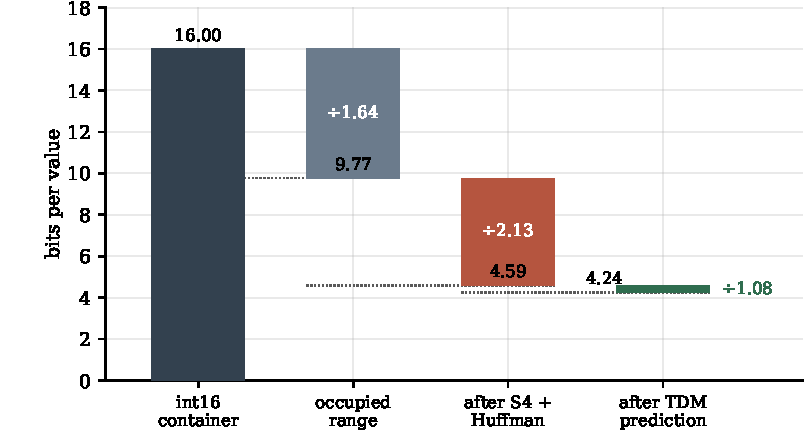
\includegraphics[width=0.66\textwidth]{fig_waterfall.pdf}
\captionof{figure}{Decomposition of the compression ratio. Of the 16 bits in the
\texttt{int16} container, 6.2 are structurally unused; the entropy coder
recovers 2.13 from spectral sparsity; corrected prediction adds 1.08.}
\end{minipage}
\end{center}

\begin{center}
\begin{minipage}{0.98\textwidth}\centering
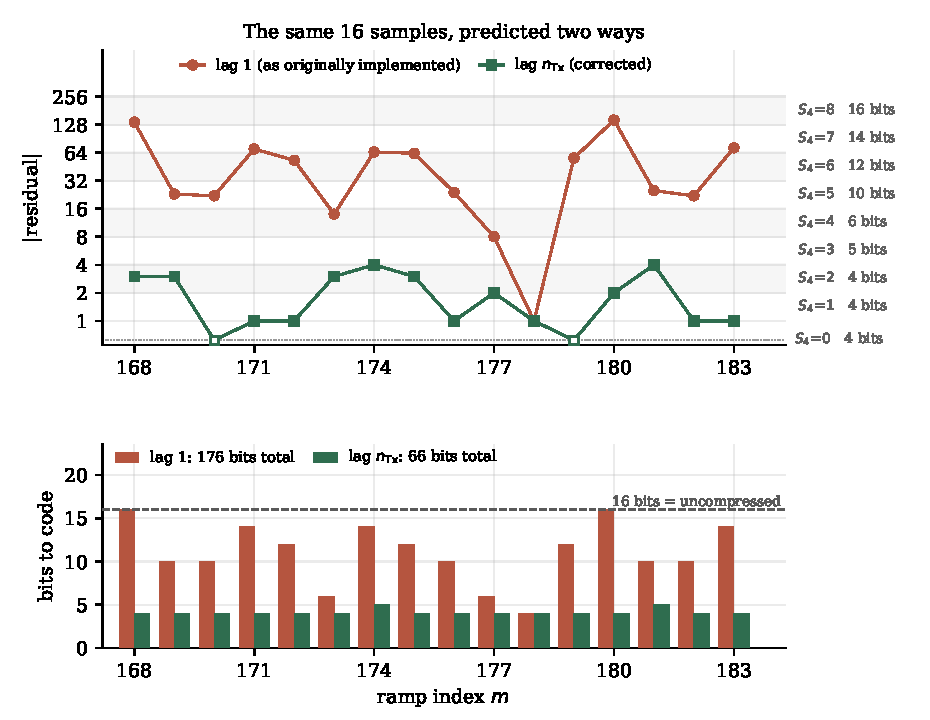
\includegraphics[width=0.90\textwidth]{fig_worked.pdf}
\captionof{figure}{The 16-sample worked example plotted. Above: residual magnitude with
the S4 cost bands marked. Below: bits per sample against the 16 uncompressed.
176 bits versus 66, for identical information.}
\end{minipage}
\end{center}

\begin{center}
\begin{minipage}{0.98\textwidth}\centering
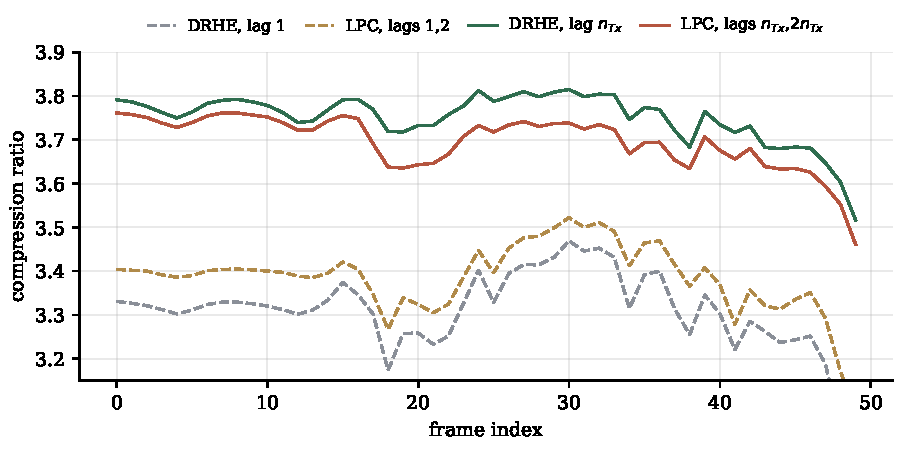
\includegraphics[width=0.92\textwidth]{fig_perframe.pdf}
\captionof{figure}{Per-frame compression ratio, all 50 frames. The corrected designs
(solid) beat their baselines (dashed) on every frame, not just on average.}
\end{minipage}
\end{center}

\begin{center}
\begin{minipage}{0.98\textwidth}\centering
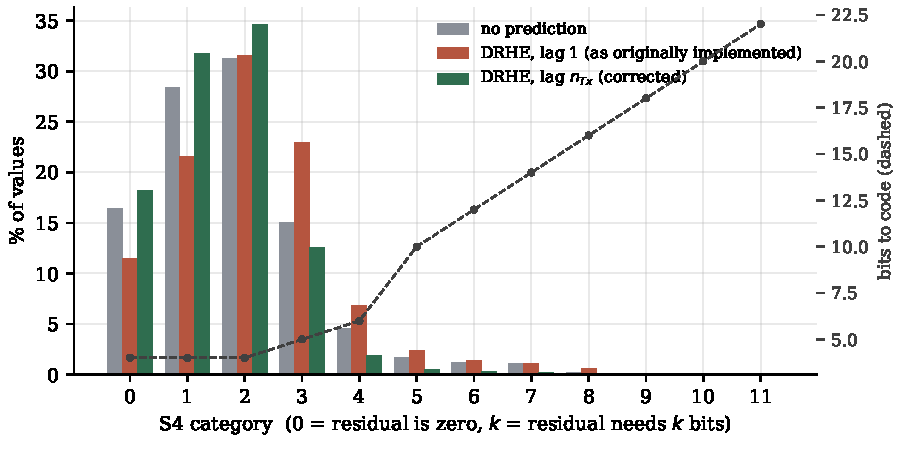
\includegraphics[width=0.92\textwidth]{fig_s4compare.pdf}
\captionof{figure}{S4 category distribution. Lag-1 prediction pushes values \emph{up} the
cost scale relative to no prediction; lag-$n_{\mathrm{Tx}}$ pulls them back down.}
\end{minipage}
\end{center}

\begin{center}
\begin{minipage}{0.98\textwidth}\centering
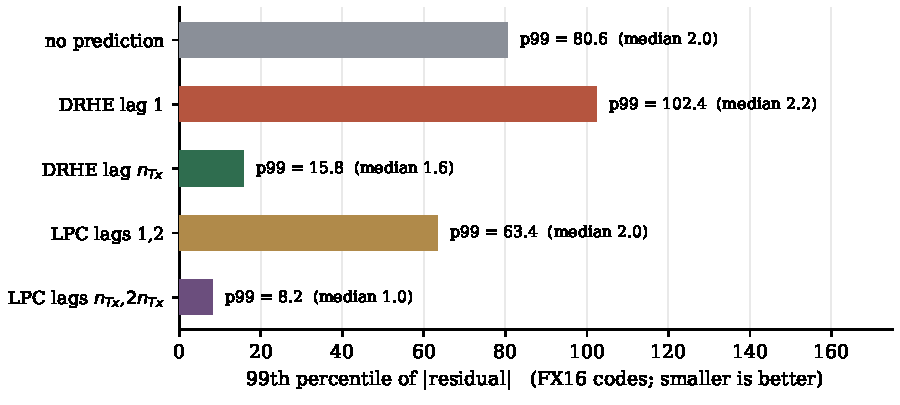
\includegraphics[width=0.88\textwidth]{fig_residmag.pdf}
\captionof{figure}{99th percentile of residual magnitude --- the clearest single view.
Lag-1 DRHE has a \emph{heavier} tail than no prediction at all.}
\end{minipage}
\end{center}

\begin{center}
\begin{minipage}{0.98\textwidth}\centering
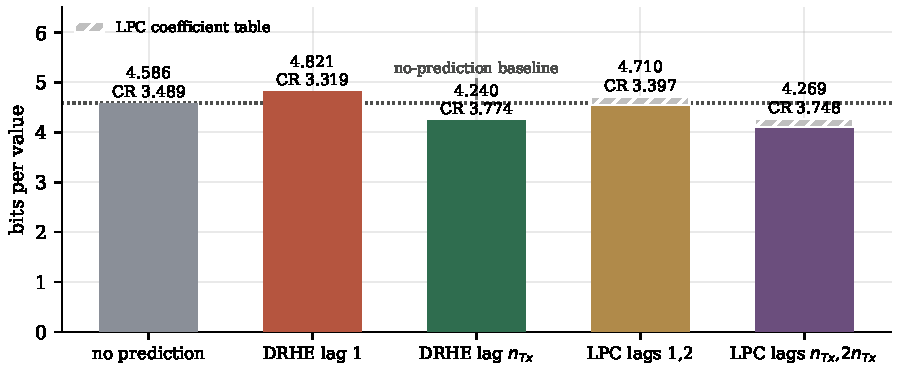
\includegraphics[width=0.92\textwidth]{fig_bpv.pdf}
\captionof{figure}{Bits per value, all five configurations. Dotted line is the
no-prediction baseline: any bar above it is a predictor doing harm.}
\end{minipage}
\end{center}

\begin{center}
\begin{minipage}{0.98\textwidth}\centering
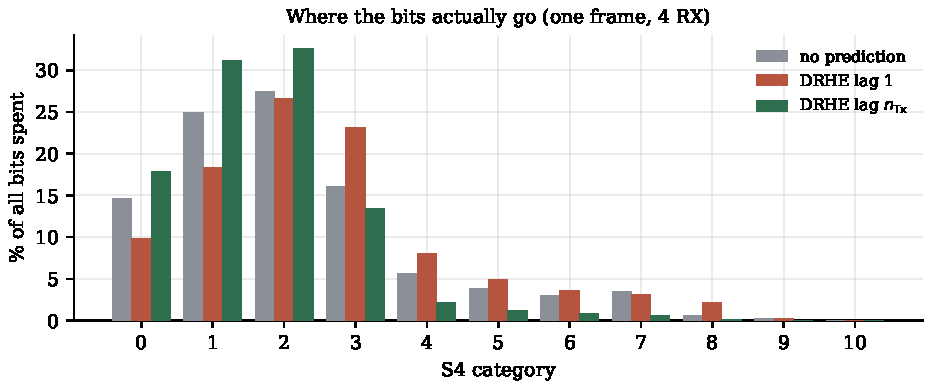
\includegraphics[width=0.92\textwidth]{fig_bitbudget.pdf}
\captionof{figure}{Share of total bits by S4 category. The correction concentrates
spending into the three four-bit categories.}
\end{minipage}
\end{center}

\begin{center}
\begin{minipage}{0.98\textwidth}\centering
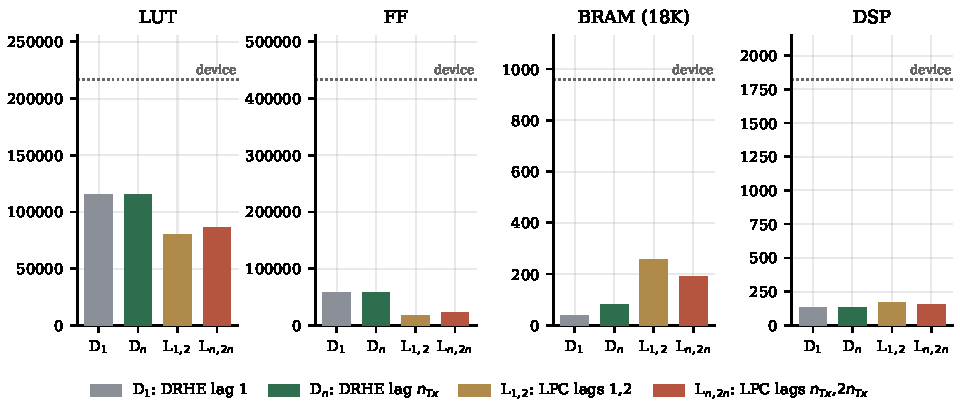
\includegraphics[width=\textwidth]{fig_resources.pdf}
\captionof{figure}{Resource usage, four designs, against device capacity (dotted). DRHE
trades block RAM for logic; LPC the reverse.}
\end{minipage}
\end{center}

\end{document}
